\documentclass[10pt,a4paper]{article}
\usepackage{amsmath,amssymb,amsthm,graphicx}
\usepackage{fontspec}
\setmainfont{DejaVu Serif}
\usepackage{amsmath,amssymb,amsthm,graphicx,xcolor}
\usepackage[unicode,hidelinks]{hyperref}
\usepackage[a4paper,margin=25mm]{geometry}
\newtheorem{theorem}{Theorem}[section]
\newtheorem{lemma}[theorem]{Lemma}
\newtheorem{corollary}[theorem]{Corollary}
\newtheorem{claim}[theorem]{Claim}
\newtheorem{proposition}[theorem]{Proposition}
\newtheorem{observation}[theorem]{Observation}
\theoremstyle{definition}
\newtheorem{definition}[theorem]{Definition}
\newtheorem{example}[theorem]{Example}
\graphicspath{{items/}}
\usepackage{cleveref}
\crefname{originalcorollary}{original corollary}{original corollarys}
\Crefname{originalcorollary}{Original corollary}{Original corollarys}
\makeatletter
\newlabel{cor:kmrr}{{1.3}{source}{}{sourcepointer-1}{}}
\newlabel{cor:kmrr@cref}{{[originalcorollary][0][]1.3}{[1][0][]source}{}{}{}}
\makeatother
\crefname{originalproposition}{original proposition}{original propositions}
\Crefname{originalproposition}{Original proposition}{Original propositions}
\makeatletter
\newlabel{iterated 2}{{3.3}{source}{}{sourcepointer-2}{}}
\newlabel{iterated 2@cref}{{[originalproposition][0][]3.3}{[1][0][]source}{}{}{}}
\makeatother
\crefname{originalproposition}{original proposition}{original propositions}
\Crefname{originalproposition}{Original proposition}{Original propositions}
\makeatletter
\newlabel{linear proof}{{4.3}{source}{}{sourcepointer-3}{}}
\newlabel{linear proof@cref}{{[originalproposition][0][]4.3}{[1][0][]source}{}{}{}}
\makeatother
\crefname{originalproposition}{original proposition}{original propositions}
\Crefname{originalproposition}{Original proposition}{Original propositions}
\makeatletter
\newlabel{prop iterated full}{{4.5}{source}{}{sourcepointer-4}{}}
\newlabel{prop iterated full@cref}{{[originalproposition][0][]4.5}{[1][0][]source}{}{}{}}
\makeatother
\crefname{originaltheorem}{original theorem}{original theorems}
\Crefname{originaltheorem}{Original theorem}{Original theorems}
\makeatletter
\newlabel{thm:main}{{1.2}{source}{}{sourcepointer-5}{}}
\newlabel{thm:main@cref}{{[originaltheorem][0][]1.2}{[1][0][]source}{}{}{}}
\makeatother
\title{Infinite polynomial sum-product boosting for geometric Ramsey families}
\author{Matt Bowen}
\date{arxiv2210.14311v3; CC BY 4.0 (fixed arXiv v3 metadata, native author TeX and figures); CC BY 3.0 (original PDF embedded journal-template link)}
\begin{document}
\maketitle
\setcounter{section}{1}
\setcounter{theorem}{0}
\noindent\textit{Editorial scope.} Count exactly the complete geometric-family boosting theorem, Proposition 4.1 (geo proof), as one independent H2 problem. Its arbitrary finite coloring and polynomial-space parameters, arbitrary geometric Ramsey family, infinite A and mixed product/shift conclusion are kept intact. Include the entire Claim 4.2 construction and the explicitly referenced complete geometric concrete-case construction, Claim 3.2, with Figure 1. Do not count Theorem 1.2, the linear or iterated cases, any supporting claim, Proposition 3.1, or any application corollary.\par\medskip
\noindent\textit{Editorial note.} All mathematical text is the native fixed author v3 source. Supporting constructions are retained, not counted separately. No generated proof, additional hypothesis or mathematical correction is supplied.\par\medskip
\noindent\textit{Editorial note.} Theorem 1.2 is not counted here: v3 leaves the current linear and iterated tree modifications explicitly omitted; v1 and v2 do too. Only the separately stated and completely written geometric-family proposition is selected.\par\medskip
\noindent\textit{Editorial note.} The standard article wrapper preserves original section/theorem counters. Figure 1 is the unchanged original PNG, displayed with bounded dimensions and its entire original caption. The original bibliography is retained in order.\par\medskip
\noindent\textit{Editorial note.} The fixed arXiv v3 metadata and journal page show CC BY 4.0; the original PDF template links CC BY 3.0. Both notices are retained and disclosed; publisher classes and email-icon assets remain private.\par\medskip
\noindent\textit{Editorial note.} This is author-material collection, not an independent mathematical review. The source text and original source-level notation/cross-references are not repaired.\par\medskip
\noindent\textit{Editorial scope.} Count exactly the complete geometric-family boosting theorem, Proposition 4.1 (geo proof), as one independent H2 problem. Its arbitrary finite coloring and polynomial-space parameters, arbitrary geometric Ramsey family, infinite A and mixed product/shift conclusion are kept intact. Include the entire Claim 4.2 construction and the explicitly referenced complete geometric concrete-case construction, Claim 3.2, with Figure 1. Do not count Theorem 1.2, the linear or iterated cases, any supporting claim, Proposition 3.1, or any application corollary.\par\medskip
\noindent\textit{Allowed standard prerequisites (editorial).}\begin{itemize}
\item Polynomial van der Waerden theorem for commutative semigroups. Author Theorem 2.4 gives the exact piecewise-syndetic P\_n variant and rational-denominator explanation; original references [4] Bergelson–Leibman (1996) and [3] Bergelson–Glasscock Theorem 7.8.. A standard external recurrence tool; the current tree parameter sets, nested color refinements and extraction proof remain fully in the item.
\item Partition regularity of piecewise-syndetic sets. Author Lemma 2.3; original [10] Hindman–Strauss (2011), Theorem 4.4.. Choose piecewise-syndetic color classes before multiplication; the source-specific use and construction are retained.
\item Finite coloring compactness, pigeonhole principle, Schur/Rado background and basic polynomial/set operations. Standard Ramsey prerequisites; the source includes exact Ramsey-family, tree and polynomial-space definitions.. Obtain finite pattern sets and repeated colors; no geometric-family color-focusing core is assumed as a prerequisite.
\end{itemize}\medskip
\ifdefined\hypertarget\hypertarget{sourcepointer-1}{}\fi
\noindent\textit{Source reference.} Original corollary 1.3: persistence-modules/\allowbreak{}arxiv2210.14311/\allowbreak{}sources/\allowbreak{}arxiv2210.14311v3/\allowbreak{}main\_formatted.tex, source lines 141--143. Descriptive author reference to a different result or example; it is not invoked to prove the counted geometric-family proposition. The counted proposition and its entire current construction are included directly.\par\medskip
\ifdefined\hypertarget\hypertarget{sourcepointer-2}{}\fi
\noindent\textit{Source reference.} Original proposition 3.3: persistence-modules/\allowbreak{}arxiv2210.14311/\allowbreak{}sources/\allowbreak{}arxiv2210.14311v3/\allowbreak{}main\_formatted.tex, source lines 352--354. Descriptive author reference to a different result or example; it is not invoked to prove the counted geometric-family proposition. The counted proposition and its entire current construction are included directly.\par\medskip
\ifdefined\hypertarget\hypertarget{sourcepointer-3}{}\fi
\noindent\textit{Source reference.} Original proposition 4.3: persistence-modules/\allowbreak{}arxiv2210.14311/\allowbreak{}sources/\allowbreak{}arxiv2210.14311v3/\allowbreak{}main\_formatted.tex, source lines 472--474. Descriptive author reference to a different result or example; it is not invoked to prove the counted geometric-family proposition. The counted proposition and its entire current construction are included directly.\par\medskip
\ifdefined\hypertarget\hypertarget{sourcepointer-4}{}\fi
\noindent\textit{Source reference.} Original proposition 4.5: persistence-modules/\allowbreak{}arxiv2210.14311/\allowbreak{}sources/\allowbreak{}arxiv2210.14311v3/\allowbreak{}main\_formatted.tex, source lines 500--506. Descriptive author reference to a different result or example; it is not invoked to prove the counted geometric-family proposition. The counted proposition and its entire current construction are included directly.\par\medskip
\ifdefined\hypertarget\hypertarget{sourcepointer-5}{}\fi
\noindent\textit{Source reference.} Original theorem 1.2: persistence-modules/\allowbreak{}arxiv2210.14311/\allowbreak{}sources/\allowbreak{}arxiv2210.14311v3/\allowbreak{}main\_formatted.tex, source lines 114--131. Descriptive author reference to a different result or example; it is not invoked to prove the counted geometric-family proposition. The counted proposition and its entire current construction are included directly.\par\medskip
Ramsey theory on $\mathbb{N}$ is centered around characterizing the structures of the following form.

\begin{definition}
\normalfont We say a family $\mathcal{B}\subseteq \mathcal{P}(\mathbb{N})$ is \textbf{Ramsey} if for any finite coloring $c:\mathbb{N}\rightarrow [r]$ there is some $B\in \mathcal{B}$ such that $c$ is constant on $B$. 
\end{definition}


The \textbf{linear Rado families}, i.e. the Ramsey families $\mathcal{B}$ that are generated by the set of solutions to a finite system of linear equations, are completely characterized by Rado's theorem \cite{rado1933studien}.  Moreover, given any such family we can obtain a \textbf{geometric Rado family} by composing a given coloring with the homomorphism $n\mapsto 2^n$. 
For example, Schur's theorem tells us that $\{\{x,y,z\}:x+y=z\}$ is a linear Rado family, which in turn implies that $\{\{x,y,z\}:xy=z\}$ is a geometric Rado family.  We will sometimes simply write, for example, that $\{x,y,x+y\}$ is Ramsey, a slight abuse of notation.

In contrast to the linear and geometric case, characterizations of other Ramsey families are still quite elusive, and determining if even some of the simplest non-linear families are Ramsey has been the subject of much recent study; see, e.g., \cite{alweiss2023monochromatic,alweiss2024monochromatic,chow2021rado,di2018ramsey,di2022monochromatic,moreira2017monochromatic,prendiville2021counting,sahasrabudhe2018exponential,sahasrabudhe2018monochromatic}, for some recent results of this type.  Here we further this line of work by showing that certain non-linear compositions of Ramsey families are still Ramsey.  In the below, by $\binom{\mathbb{N}}{m}$ we mean the family of all $m$-element subsets of $\mathbb{N},$ while $\binom{\mathbb{N}}{\infty}$ is the family of all infinite subsets of $\mathbb{N}.$

\section{Notation and technical background}

In this section we collect the notation and technical facts that will be used throughout the paper.  The reader should note that the proofs of the special cases of our main result presented in Section \ref{concrete}, which contain almost all of the combinatorial ideas needed for the proof of our general theorem, mostly avoid these notations and rely on more well known facts.  Namely, the only thing from Subsection \ref{subsection poly} needed in Section \ref{concrete} is the more usual $\mathbb{P}_0=\mathbb{N}$ case of the polynomial van der Waerden theorem, and Subsection \ref{subs family} can be entirely skipped.

The main technical difficulty with the proof of Theorem \ref{thm:main} is that each step of our induction will require us to prove Ramsey theoretic results on the space of polynomials with an additional variable (see the discussion after the proof of Theorem \ref{iterated 2}), which leads to notational difficulties if not combinatorial ones.  

Throughout, we will often abuse notation when using algebraic operations with sets.  For example, if $A$ and $B$ are sets of numbers, by $\frac{A}{B}$ we mean the set $\{\frac{a}{b}:a\in A, b\in B\}.$  Similarly, if $P$ and $Q$ are sets of polynomials, by $P(d)$ we mean the set $\{p(d):p\in P\}$ and by $Q(P(d))$ we mean the set $\{q(p(d)): q\in Q,p\in P\}.$

\subsection{Trees}

In this paper, by a \textbf{tree} we mean a collection of finite words (including the empty word) where the $n$th letter comes from alphabet $A_n.$  More precisely, given finite sets $A_0,...,A_R,$ we'll consider trees of the form $T=\bigcup_{0\leq i\leq R+1}\prod_{j<i} A_j. $  In particular, $T$ is rooted at the empty word, which has $|A_0|$ children each labeled by an element of $A_0$, and so on.

Given a tree $T$ as above, we define the $i$th level of the tree as $T_i=\prod_{j<i} A_j.$  Further, we will use $\smallfrown$ to denote concatenation, i.e., given $t\in T_i$ and $p\in A_i,$ $t\smallfrown p\in T_{i+1}.$

\subsection{Polynomial spaces, notions of size, and van der Waerden's theorem}\label{subsection poly}

As mentioned above, the proof of Theorem \ref{thm:main} will require us to consider spaces of many variabled polynomials with rational coefficients.

\begin{definition}
Let $\mathbb{P}_0=\mathbb{N},$ and having defined $\mathbb{P}_n,$ let $\mathbb{P}_{n+1}$ be the set of all formal objects of the form $\frac{a_1}{b_1}x_{n+1}+\frac{a_2}{b_2}x_{n+1}^2+...+\frac{a_k}{b_k}x_{n+1}^k,$ where $x_{n+1}$ is a formal variable different from the ones used to define $\mathbb{P}_n,$ $k\in\mathbb{N}$, and $a_j,b_j\in \bigcup_{0\leq i\leq n} \mathbb{P}_i,$ and $b_j\neq 0.$ 
\end{definition}


In particular, $\mathbb{P}_1=x\mathbb{Q}_+[x],$ the space of all formal polynomials of degree at least one with positive rational coefficients together with the $0$-polynomial $n\mapsto 0$. 

Given $p\in \mathbb{P}_{n}$ and $d\in\mathbb{P}_m,$ by $p(d)$ we mean the formal object obtained by replacing every instance of $x_{n}$ in $p$ with $d.$  We will only do this in instances where $m=n,$ in which case this is the composition of polynomials, or when $m=n-1,$ where we can think of this as evaluation.  Note that in the latter case in general this might not be an element of $\mathbb{P}_{n-1},$ but in all of our uses of this notation $d$ will have been chosen such that it is.

We will need a piecewise syndetic version of the polynomial van der Waerden theorem for our proofs. To formally state this, we need the following definitions.  


\begin{definition}
\hspace{3mm}
\begin{itemize}
    \item A set $S\subseteq \mathbb{P}_n$ is \textbf{syndetic} if there is a finite set $F\subset\mathbb{P}_n$ such that $\mathbb{P}_n\subseteq S-F.$
    
    \item A set $T\subseteq\mathbb{P}_n$ is \textbf{thick} if for any finite set $F,$ there is a $t\in T$ such that $t+F\subset T.$
    
    \item  A set $A\subseteq\mathbb{P}_n$ is \textbf{piecewise syndetic} if there is a thick set $T$ and a syndetic set $S$ with $S\cap T\subseteq A.$
\end{itemize}
\end{definition}  

Unlike for $\mathbb{N},$ $x_{n}\mathbb{P}_n$ is not piecewise syndetic for $n>0.$  This was mentioned by Moreira in \cite{moreira2017monochromatic} Section 7 as a difficulty with extending his proof to rings that are not large ideal domains (such as $\mathbb{P}_n$ for $n>0)$.  However, this fact will not be problematic for us, since we will frontload our use of lemmas about piecewise syndetic sets to before we do any multiplications in all of our proofs.

We now state the two facts about piecewise syndetic sets that we will need.  The first is well known; see, e.g. \cite{hindman2011algebra}, Theorem 4.4.

\begin{lemma}\label{lemma tech}
If $A\subseteq \mathbb{P}_n$ is piecewise syndetic and $A=A_0\cup...\cup A_R,$ then some $A_i$ is piecewise syndetic.
\end{lemma}

Finally, we will use the following variant of the Polynomial van der Waerden theorem.

\begin{theorem}[Polynomial van der Waerden, essentially \cite{bergelson1996polynomial}]\label{pvd}
Let $P\subset \mathbb{P}_{n+1}$ be a finite set of polynomials and $A\subseteq\mathbb{P}_n$ be piecewise syndetic.  Then there is some $d\in\mathbb{P}_n$ such that $$A\cap \bigcap_{p\in P}(A-p(d))$$ is piecewise syndetic.

\end{theorem}

This follows from any variant of the polynomial van der Waerden theorem for commutative semigroups, such as \cite{bergelson2016interplay} Theorem 7.8.  Note that the presence of rational rather than the integral coefficients more typically discussed in this context does not lead to any difficulties.  For example, the existence of monochromatic progressions of the form $a,a+d, a+\frac{d}{2}, a+\frac{d}{3}$ follows from the existence of monochromatic progressions of the form $a, a+2d', a+3d', a+6d'$ and setting $d=6d'.$


\subsection{Ramsey families}\label{subs family}

We will use the following generalization of the linear and geometric Rado families discussed in the introduction.  This generality is mostly present just to isolate the properties of the Ramsey families that are needed for the proof; that is, these are the properties that will be used to glue two Ramsey families together in a way that preserves their structure.

\begin{definition}\label{def ramsey}
Let $\mathcal{B}$ be a family of finite subsets of $\mathbb{P}_n.$
\begin{itemize}
    \item $\mathcal{B}$ is \textbf{$\mathbb{P}_n$-Ramsey} if for any finite coloring $c:\mathbb{P}_n\rightarrow [R]$ there is a $B\in\mathcal{B}$ such that $c$ is constant on $B.$ 
    \item $\mathcal{B}$ is a \textbf{linear Ramsey family} if it is Ramsey and if for every $B\in\mathcal{B}$ and $c\in \mathbb{P}_n,$ $cB\in \mathcal{B}.$
    \item $\mathcal{B}$ is a \textbf{geometric Ramsey family} if it is Ramsey and every $B,C\in\mathcal{B}$ can be expressed as $B=(b_0,...,b_m),$ $C=(c_0,...,c_m)$, where also $(b_0c_0,...,b_mc_m)\in \mathcal{B}.$ Here we insist that this ordering is consistent between elements (for example, the like terms in geometric progressions).
\end{itemize}
\end{definition}

Observe that every linear Rado family is a linear Ramsey family in $\mathbb{P}_n,$ which can be seen by considering the polynomials of the form $\{ix_{n}: i\leq k\}$ for sufficiently large $k,$ and every geometric Rado family is a geometric Ramsey family in $\mathbb{P}_n$ by considering polynomials of the form $\{x_{n}^i: i\leq k\}.$  Throughout this paper we will only be interested in linear and geometric Ramsey families of this form, so we do not specify if they are $\mathbb{P}_n$ Ramsey or $\mathbb{P}_{n+1}$ Ramsey.  This will only be relevant in the proofs of Propositions \ref{geo proof} and \ref{linear proof}. 

The following are representative examples of each type of Ramsey family that is in $\mathbb{T}$ and thus can be composed as in Theorem \ref{thm:main}.  

\begin{example}

\hspace{2mm}
    \begin{enumerate}
        \item The family $\{\{x,y, x+y\}: x,y\in\mathbb{N}\}$ is a linear Ramsey family.  Examples such as this will be analyzed in Proposition \ref{linear proof}.

        \item The family $\mathcal{B}=\{\{x,y,xy^i: i\leq k\}: x,y\in \mathbb{N}\}$ is a geometric family: if $\{x_0,y_0,x_0y_0^i:i\leq k\}$ and $\{x_1,y_1,x_1y_1^i:i\leq k\}$ are in $\mathcal{B}$ then so is $\{x_0x_1, y_0y_1, (x_0x_1)(y_0y_1)^i: i\leq k\}$.  However, it is not a linear Ramsey family.  Examples such as this will be analyzed in Propositions \ref{geom2} and \ref{geo proof}.

        \item The family $\{\{x+y, xy\}: x,y\in\mathbb{N}\}$ is neither linear nor geometric.  However, it is still a member of $\mathbb{T},$ and examples such as this will be analyzed in Propositions \ref{iterated 2} and \ref{prop iterated full}.  
    \end{enumerate}
\end{example}

We will also use the following fact about geometric Ramsey families.

\begin{observation}\label{obs tech}
    Let $\mathcal{B}$ be a geometric Ramsey family and $B_0,...,B_R\in\mathcal{B},$ where we can write $B_i=(b_{0,i},\ldots,b_{m,i})$.  Then defining $b_j=b_{j,0}\cdot b_{j,1}\ldots\cdot b_{j,R}$ for each $j\in \{0,\ldots,m\}$ and $B=\{b_0,\ldots,b_m\},$ we have that $B\in \mathcal{B}$.
\end{observation}

\begin{proof}
    This follows from the definition of being geometric and induction on $R.$ 
    \end{proof}

\section{Two concrete cases}\label{concrete}

In this section we prove two special cases of our main result that contain essentially all of the ideas needed for the general Theorem \ref{thm:main} while requiring much less notation.  Our first example is the following.

\begin{proposition}\label{geom2}
Any $2$-coloring of $\mathbb{N}$ contains a monochromatic set of the form $$\{a,ab,ac,abc, a+b,a+c,a+bc\}.$$
\end{proposition}

This is the two color case of Theorem \ref{thm:main} applied to the geometric Ramsey family $\{b,c,bc\}$ and the polynomials $n\mapsto 0$ and $n\mapsto n$.  The proof here generalizes easily to more colors and arbitrary geometric Ramsey families and polynomials, although we save the details for the next section for the sake of clarity and simplicity of notation.  In particular, the methods here can be easily adapted to prove Corollary \ref{cor:kmrr}.


\begin{proof}
Suppose that $\mathbb{N}=C_0\cup C_1.$  Our goal is to build a tree of infinite sets with edges labeled by polynomials that we will use for a color focusing argument.  

\begin{claim}\label{geo simple claim}
There are finite sets of polynomials $P_0,P_1\subset \mathbb{P}_1,$ elements $d_0,d_1\in \mathbb{N},$ and a tree of infinite monochromatic sets $A_t\subseteq \mathbb{N}$ for $t\in T=\bigcup_{0\leq i\leq 2}\prod_{j<i}P_{j}$ such that
\begin{enumerate}
    \item any $2$-coloring of ${P}_{1}$ contains a monochromatic set of the form $\{b,c,bc\}$ (in this case, $P_1=\{x^i: i\leq s\},$ where $s$ is the $2$-color Schur number, would work).

    \item any $2^{|P_{1}|+1}$-coloring of $P_0$ contains a monochromatic set of the form $\{b,c,bc\}.$
    
    \item  for each $t\in T_i$ there is an $r\in \{0,1\}$ such that $A_t\cup\bigcup_{k\geq i}(A_t+\prod_{i\leq j\leq k}P_j(d_j))\subseteq C_r.$

    \item for $t\in T_i$ and $p_i\in P_i$ we have $p_i(d_i)A_t=A_{t\smallfrown p_i}.$
\end{enumerate}
\end{claim}

\vspace{2mm}

We will call structures similar to the one described above \textbf{color focusing trees}.  Before proving the claim, let us see how to use it to finish the proof of Proposition \ref{geom2} (see, especially, Figure \ref{fig:focusing1}). 

\begin{figure}
    \centering
    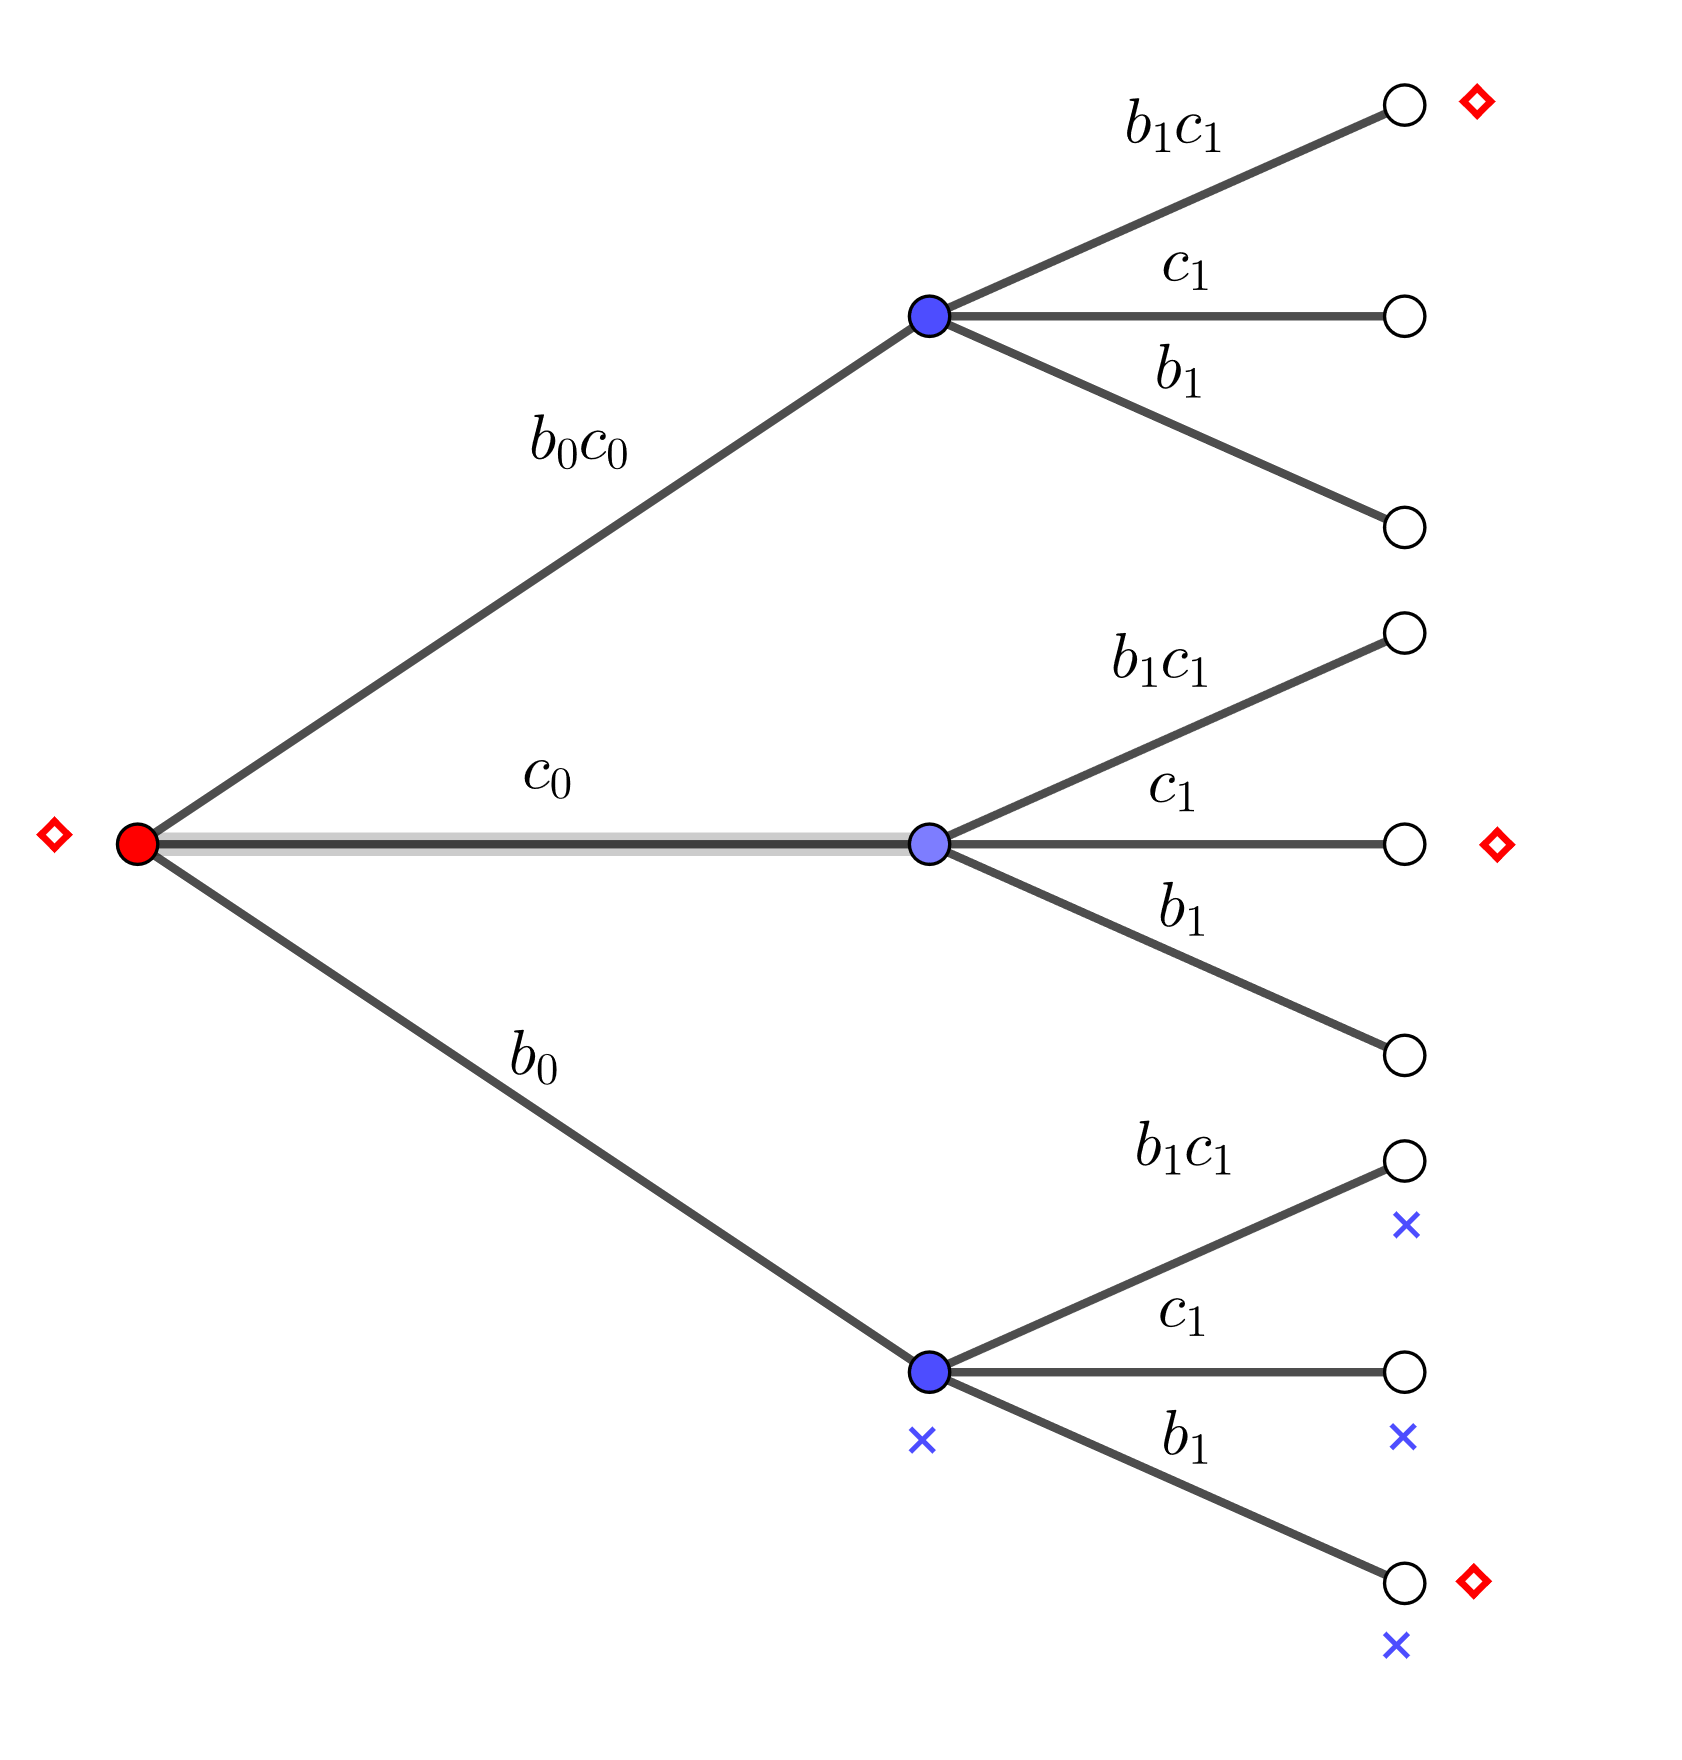
\includegraphics[width=0.85\linewidth,height=0.70\textheight,keepaspectratio]{focusing_1_marked.png}
    \caption{The color focusing step of the proof of Proposition \ref{geom2}.  Each vertex of the tree represents an infinite monochromatic set and multiplying by the indicated polynomials sends elements of a vertex to its child.  The uncolored vertices are all the same color.  If these vertices are blue then we can finish the proof by setting $b={b_1}(d_1)$ and $c={c_1}(d_1)$ and considering the vertices marked with ${\color{blue} \times}.$  Otherwise they are red and we can finish by setting $b={b_0}(d_0)\cdot b_1(d_1)$ and $c={c_0}(d_0)\cdot {c_1}(d_1)$ and considering the vertices marked with ${\color{red} \diamondsuit}.$}
    \label{fig:focusing1}
\end{figure}

Without loss of generality we may assume that $A_\emptyset\subseteq C_0.$  Note also that by Property (3) of Claim \ref{geo simple claim} that each set $A_t$ for $t\in T$ is monochromatic, and hence we can $2$-color the $t\in T$ based on the color of $A_t$.  Now, consider an auxiliary $2^{|P_1|+1}$-coloring of the $p\in P_0$ based on the $(|P_1|+1)$-tuple consisting of the color of $A_p$ together with the colors of its $|P_1|$ descendants in the tree.  By Property (2) of the Claim we find $b_0,c_0\in P_0$ such that the set $P_0'=\{{b_0}, {c_0}, {b_0c_0}\}$ is monochromatic according to this coloring.  By Property (4) of the Claim, this means that for any $a_0\in A_\emptyset$ the set $\{a_0p(d_0): p\in P'_0\}$ is monochromatic.

If this set is monochromatic in $C_0$ then we can finish the proof by letting $a\in A_\emptyset\subseteq C_0,$ $b={b_0(d_0)},$ and $c={c_0(d_0)}.$ This is because $\{ab,ac,abc\}\subset C_0$ by the above paragraph and $\{a+b,a+c,a+bc\}\subset A_\emptyset+P_0(d_0)\subseteq C_0$ by Property (3) of the Claim.

Otherwise, we can assume that $A_{p}\subseteq C_1$ for each $p\in P_0'.$  By our construction, for $p_1\in P_1$ and $p'_0
\in P_0',$ the color of $p_1(d_1)A_{p'_0}$ depends only on $p_1.$  Considering the $2$-coloring of $p\in P_1$ based on the color of $A_{p'\smallfrown p}$ and using Property (1) of the claim, we find $b_1,c_1\in P_1$ such that $P_1'=\{{b_1}, {c_1}, {b_1c_1}\}$ is monochromatic.  This means that the sets $A_{p'_0\smallfrown p'_1}$ for $p'_0\in P'_0$ and $p'_1\in P'_1$ are all monochromatic in the same color.

If $p'_1(d_1)A_{p_0'}\subseteq C_1$ for $p'_1\in P'_1$ and $p'_0\in P'_0,$ then we can finish as above by taking $a\in A_{p_0'},$ $b={b_1(d_1)},$ $c={c_1(d_1)}$, and applying Properties (3) and (4) of the Claim as done above.

Otherwise, $p'_1(d_1)A_{p_0'}\subseteq C_0$ for $p'_1\in P'_1$ and $p'_0\in P'_0.$  In this case we can finish by setting $a\in A_\emptyset,$ $b={b_0}(d_0)\cdot {b_1(d_1)},$ and $c={c_0(d_0)}\cdot {c_1(d_1)},$ and applying Properties (3) and (4) of the Claim as above.



Now, in order to finish the proof of Proposition \ref{geom2} we just need to prove Claim \ref{geo simple claim}.

\begin{proof}[Proof of Claim \ref{geo simple claim}]
The construction of the sets $A_t$ is routine and follows from a couple of applications of the polynomial van der Waerden theorem.  If we were interested in finding a sequence rather than a tree of infinite sets satisfying the conditions of the Claim, then the construction would be essentially the same as that used by Moreira in \cite{moreira2017monochromatic} Corollary 1.5.

First we define $P_1$ and $P_0.$ Let $s_1$ be the $2$-color Schur number and define $P_1=\{x^i: i\leq s_1\}.$  Let $s_0$ be the $2^{s_1+1}$-color Schur number and $P_0=\{x^i: i\leq s_0\}.$  These satisfy properties (1) and (2).

Now, without loss of generality we may assume that $C_0$ is piecewise syndetic by Lemma \ref{lemma tech}.  By Theorem \ref{pvd}, we know that there is a $d_0\in \mathbb{N}$ such that the set $A_0=C_0\cap\bigcap_{p\in P_0} (C_0-p(d_0))$ is piecewise syndetic.  Consider the $2^{|P_0|}$-coloring of $a_0\in A_0$ based on the $|P_0|$-tuple listing the colors of $a_0\cdot p_0(d_0)$ for $p_0\in P_0.$  By Lemma \ref{lemma tech}, one of these color classes is piecewise syndetic.  Let this set be $A_0'.$

Apply Theorem \ref{pvd} to $A'_0$ with the set of polynomials $$P_1'=\{p_0(d_0) p_1,\frac{p_1}{p_0(d_0)}: p_i\in P_i\} $$ to find $d_1\in \mathbb{N}$ such that $A_1=A_0'\cap\bigcap_{p_1\in P_1'} (A_0'-p_1(d_1))$ is piecewise syndetic.  Finally, consider the $2^{|P_0|\cdot|P_1|}$ coloring of the $a_0\in A_1$ based on the tuple listing the color of $a_0\cdot p_0(d_0)\cdot p_1(d_1),$ and let $A_\emptyset$ be the color class that is piecewise syndetic by Lemma \ref{lemma tech}.  Letting $A_t$ be defined to satisfy Property (4) of the claim gives the desired sets.
\end{proof}



\end{proof}

\section{The general case}

In this section we prove Theorem \ref{thm:main}.  As mentioned previously, all of the combinatorial ideas needed for the proof are already present in the two concrete cases discussed in Section \ref{concrete}, so we suggest that the reader focus on understanding those proofs.  We only include the technical proofs in this section for the purpose of completeness and verification.

The proof will split into three independent cases depending on the structure of the family $\mathcal{B}$.  Throughout we will need to work in the space of many variabled rational polynomials for the reasons discussed after the proof of Proposition \ref{iterated 2}.  

\begin{proposition}\label{geo proof}
Let $\mathbb{P}_n=C_1\cup...\cup C_R$ be a finite coloring, $P\subset \mathbb{P}_{n+1}$ a finite set of polynomials, and $\mathcal{B}$ a geometric Ramsey family.  There is an infinite $A\subseteq \mathbb{P}_n$ and a $B\in\mathcal{B}$ such that $$\{a,ab,a+p(b): a\in A, b\in B, p\in P\}$$ is monochromatic.  
\end{proposition}

\begin{proof}


As in the special cases proved in Section \ref{concrete}, our goal is to build a color focusing tree.

\begin{claim}\label{geo}
There are finite sets of polynomials $P_0,...,P_R\subset \mathbb{P}_{n+1},$ elements $d_0,...,d_R\in \mathbb{P}_n,$ and a tree of infinite monochromatic sets $A_t$ for $t\in T=\bigcup_{0\leq i\leq R+1}\prod_{j<i}P_{j}$ such that

\begin{enumerate}
    \item any $R$-coloring of ${P}_{R}$ contains a monochromatic element of $\mathcal{B}.$
    \item for $0\leq i<R,$ any $R^{|P_{i+1}|\cdot...\cdot|P_R|+1}$-coloring of $P_i$ contains a monochromatic element of $\mathcal{B}.$
    \item  for each $0\leq i\leq R$ and each $t\in T_i$ there is a $c\in \{1,...,R\}$ such that $$A_t\cup\bigcup_{i\leq k\leq R}(A_t+P(\prod_{i\leq j\leq k}P_j(d_j)))\subseteq C_c.$$
    \item for $t\in T_i$ and $p_i\in P_i$ we have $p_i(d_i)A_t=A_{t\smallfrown p_i}.$
\end{enumerate}
\end{claim}

We can use Claim \ref{geo} to finish the proof in exactly the same manner as we finished the proof of Proposition \ref{geom2} (see especially Figure \ref{fig:focusing1}).  We include the details here more for the purpose of verification and completeness than understanding.

By coloring vertices $t\in T$ based on the color of $A_t$ and the color of all of their descendants in the tree and applying Properties (1) and (2) of Claim \ref{geo}, we find subsets $B_0\subset P_0,$ $\ldots,$ $B_R\subset P_R$ such that $B_k\in\mathcal{B}$ for $k\in \{0,...,R\}$ and such that for any sequence $b_0,b_1,\ldots, b_j$ with $b_k\in B_k$, the color of $A_{b_0\smallfrown...\smallfrown b_j}$ depends only on $j$ (and not on the choices of $b_k\in B_k$).  By the pigeonhole principle we find $i<j$ such that these colors agree on some color $c\in [R]$, i.e. the sets $A_{b_0\smallfrown...\smallfrown b_i}$ and $A_{b_0\smallfrown...\smallfrown b_j}$ are all subsets of $C_c$ for any choices of $b_k\in B_k$.  

Suppose that the sets $B_k\in\mathcal{B}$ for $k\in \{0,...,R\}$ all have cardinality $m+1$ and that $B_k$ can be written as $(b_{0,k},...,b_{m,k}),$ where the indexing is as in the definition of being a geometric Ramsey family, Definition \ref{def ramsey}.  Let $t=b_{0,0}\smallfrown...\smallfrown b_{0,i},$ where $i$ is the smaller index obtained via the pigeonhole principle in the previous paragraph.  To finish the proof we will define $A=A_t\subseteq C_c$ and for $0\leq k\leq m$ we define $b_k=b_{k,i+1}(d_{i+1})\cdot...\cdot b_{k,j}(d_j).$  Then since $\mathcal{B}$ is a geometric Ramsey family, we know $\{b_0,...,b_m\}=B\in \mathcal{B}$ by Observation \ref{obs tech}.  Moreover, by the previous paragraph and Property (4) of Claim \ref{geo} we know $ab_k\in C_c$ for any $b_k\in B$ and $a\in A.$  Finally, by Property (3) we know that $a+P(b_k)\subseteq C_c$ for each $a\in A$ and $b_k\in B,$ finishing the proof. 

\vspace{2mm}

Therefore, in order to complete the proof of Proposition \ref{geo proof} it suffices to prove Claim \ref{geo}.

\begin{proof}[Proof of Claim \ref{geo}]

All of the combinatorial ideas needed for the proof of the Claim were already in the proof of Claim \ref{geo simple claim}; the only new difficulty is the notation.   We will use several applications of the polynomial van der Waerden theorem.

First, we construct the polynomials $P_R,...,P_0\subset \mathbb{P}_{n+1}.$  By the definition of geometric Ramsey families and the compactness principle, we know that for any $k\in \mathbb{N}$ there is a finite set $F\subset \mathbb{P}_{n+1}$ such that any $k$-coloring of $F$ contains a monochromatic element of $\mathcal{B}.$  Let $P_R$ be such a finite set for $k=R,$ and having defined $P_R,P_{R-1},...,P_{i+1}$ let $P_i$ be such a set for $k=R^{|P_{i+1}|\cdot...\cdot|P_R|+1}.$  These satisfy Properties (1) and (2) of the claim.

For the other properties, suppose without loss of generality that $C_1$ is piecewise syndetic, and let $A'_{-1}=C_1.$  We inductively define a sequence of piecewise syndetic sets $A'_{-1}\supseteq A_0\supseteq A_0'\supseteq A_1\supseteq A_1'\supseteq... \supseteq A_{R}',$ elements $d_0,...,d_R\in \mathbb{P}_n,$ and finite sets of polynomials $P_0',...,P_R'\subset \mathbb{P}_{n+1}$ such that:

\begin{enumerate}
    \item[(a)] $$P_i'= \bigcup_{0\leq a\leq b\leq c<i} \frac{P(P_i\cdot\prod_{b\leq j\leq c} P_j(d_j))}{\prod_{ j' <a}P_{j'}(d_{j'})},$$ where empty products have value $1.$
    \item[(b)] $A_i=A_{i-1}'\cap\bigcap_{p'\in P_i'} (A_{i-1}'-p'(d_i)),$ where $d_i$ is chosen such that this set is piecewise syndetic.
    \item[(c)] Coloring $a\in A_i$ based on the tuple listing the colors of $a\cdot p_0(d_0)\cdot...\cdot p_i(d_i)$ for $p_j\in P_j,$ $A_i'$ is chosen to be a piecewise syndetic monochromatic subset of $A_i.$ 
\end{enumerate}

Finding sets satisfying (b) is possible by the polynomial van der Waerden theorem \ref{pvd}, and finding sets satisfying (c) is possible by Lemma \ref{lemma tech}.

Once these have been constructed, set $A_\emptyset=A_{R}'$ and define $A_t$ for $t\in T$ to satisfy (4) of Claim \ref{geo}.  Note that property (2) of the Claim follows from (b) and property (3) from (c).

\end{proof}

\end{proof}

\begin{thebibliography}{10}

\bibitem{alweiss2023monochromatic}
Ryan Alweiss.
\newblock Monochromatic sums and products over $\mathbb{Q}$.
\newblock {\em arXiv preprint arXiv:2307.08901}, 2023.

\bibitem{alweiss2024monochromatic}
Ryan Alweiss.
\newblock Monochromatic sums and products of polynomials.
\newblock {\em Discrete Analysis}, 2024.

\bibitem{bergelson2016interplay}
Vitaly Bergelson and Daniel Glasscock.
\newblock On the interplay between notions of additive and multiplicative
  largeness and its combinatorial applications.
\newblock {\em arXiv preprint arXiv:1610.09771}, 2016.

\bibitem{bergelson1996polynomial}
Vitaly Bergelson and Alexander Leibman.
\newblock Polynomial extensions of van der waerden’s and szemer{\'e}di’s
  theorems.
\newblock {\em Journal of the American Mathematical Society}, 9(3):725--753,
  1996.

\bibitem{bergelson2017ergodic}
Vitaly Bergelson and Joel Moreira.
\newblock Ergodic theorem involving additive and multiplicative groups of a
  field and patterns.
\newblock {\em Ergodic Theory and Dynamical Systems}, 37(3):673--692, 2017.

\bibitem{bowen.sabok}
Matt Bowen and Marcin Sabok.
\newblock Monochromatic products and sums in the rationals.
\newblock {\em Forum of Mathematics, Pi}, 12:e17, 2024.

\bibitem{chow2021rado}
Sam Chow, Sofia Lindqvist, and Sean Prendiville.
\newblock Rado's criterion over squares and higher powers.
\newblock {\em Journal of the European Mathematical Society}, 23(6):1925--1997,
  2021.

\bibitem{di2018ramsey}
Mauro Di~Nasso and Lorenzo~Luperi Baglini.
\newblock Ramsey properties of nonlinear diophantine equations.
\newblock {\em Advances in Mathematics}, 324:84--117, 2018.

\bibitem{di2022monochromatic}
Mauro Di~Nasso and Mariaclara Ragosta.
\newblock Monochromatic exponential triples: an ultrafilter proof.
\newblock {\em Proceedings of the American Mathematical Society},
  152(01):81--87, 2024.

\bibitem{hindman2011algebra}
Neil Hindman and Dona Strauss.
\newblock Algebra in the stone-ˇcech compactification.
\newblock In {\em Algebra in the Stone-Cech Compactification}. de Gruyter,
  2011.

\bibitem{kra2022infinite}
Bryna Kra, Joel Moreira, Florian~K Richter, and Donald Robertson.
\newblock Infinite sumsets in sets with positive density.
\newblock {\em arXiv preprint arXiv:2206.01786}, 2022.

\bibitem{moreira2017monochromatic}
Joel Moreira.
\newblock Monochromatic sums and products in $\mathbb{N}$.
\newblock {\em Annals of Mathematics}, pages 1069--1090, 2017.

\bibitem{prendiville2021counting}
Sean Prendiville.
\newblock Counting monochromatic solutions to diagonal diophantine equations.
\newblock {\em Discrete Analysis}, page 28173, 2021.

\bibitem{rado1933studien}
Richard Rado.
\newblock Studien zur kombinatorik.
\newblock 1933.

\bibitem{sahasrabudhe2018exponential}
Julian Sahasrabudhe.
\newblock Exponential patterns in arithmetic ramsey theory.
\newblock {\em Acta Arithmetica}, 182:13--42, 2018.

\bibitem{sahasrabudhe2018monochromatic}
Julian Sahasrabudhe.
\newblock Monochromatic solutions to systems of exponential equations.
\newblock {\em Journal of Combinatorial Theory, Series A}, 158:548--559, 2018.

\end{thebibliography}
\end{document}
